\subsection{GPU Accelerating \textit{k}mer Counting} \label{methods:gpu_accelerating_kmer_counting}
While several \textit{k}mer counting solutions have been developed in previous work, with at least one having support for GPU acceleration \cite{kmer_counting_tools}, most such tools are designed to solve the \textit{full} \textit{k}mer counting problem, which we described in section \ref{background:kmers_and_kmer_counting}.
Additionally in section \ref{background:kmers_and_kmer_counting}, we described how KAGE's \textit{k}mer counting step is a less compute and memory demanding problem which we defined as \textit{partial} \textit{k}mer counting.
As a reminder: we defined \textit{partial} \textit{k}mer counting as the process of only counting the observed occurences of a predefined set of \textit{k}mers in a sample.
Repurposing \textit{k}mer counting tools that are designed to solve the \textit{full} \textit{k}mer counting problem is futile if the goal is speedup.
Thus, we opted to implement our own GPU accelerated \textit{k}mer counting tool where its design is considered in the context of the \textit{partial} \textit{k}mer counting problem.

Although we had success in GPU accelerating a hash table in npstructures using CuPy, we decided to also attempt to implement a hash table directly in C++ using CUDA, Nvidia's programming platform.
This would allow for a more granular implementation as we would no longer be constrained to a solution originally designed for NumPy array functions.

\subsubsection{Implementation}
The hash table's interface needed to support three main operations: 1) \textbf{insert} - insert each \textit{k}mer found in an input array of \textit{k}mers (although only once upon initialization), 2) \textbf{count} - increment the value associated with each \textit{k}mer found in an input array of \textit{k}mers, and 3) \textbf{query} - fetch the values associated with each \textit{k}mer found in an input array of \textit{k}mers.

Common for all three operations mentioned above is that they need to adhere to an addressing and probing scheme.
Since our hash table resides on the GPU, certain common paradigms such as open hashing - where each address in the table contains a pointer to a linked-list or tree-type data structure for placing values - are immediately disqualified.
This is because GPUs, which architectures are designed for massive data parallelism, performs poorly when needing to de-reference pointers and make many strided memory accesses.
Thus, we went with a simple open addressing with linear probing scheme. 

Two arrays of equal size makes up the data structure where one array stores the table's keys (\textit{k}mers) and the other array stores its values (counts).
The keys array is an array of 64-bit unsigned integers.
The choice of using 64 bits for the keys, as opposed to \textit{i}.\textit{e}. 32, was to accomidate for larger \textit{k}mer values since 32 bits would only allow for \textit{k} up to $(32/2)-1=15$.
Using 64-bit keys increases our maximum \textit{k} size to 31, which is the default value for KAGE.
This choice also reveals a limitation of our hash table, which is that it can not support \textit{k}mers where $k>31$ in its current form.
The reason why 64 bits does not allow for \textit{k} up to 32, considering a 2-bit encoded 64-mer can be stored in a single 64-bit integer, is that the max 64-bit integer value is used as an indicator that a slot is empty in the hash table.
The values array is an array of 32-bit unsigned integers.
While 16-bit unsigned integers would suffice for our purpose of counting \textit{k}mers, the choice of using 32-bit unsigned integers instead was made because the CUDA framework does not have a readily usable implementation of the atomicAdd function for 16-bit integers.

The probing scheme we used - linear probing - describes how we solve collisions in the hash table. 
This scheme is shared for all three operations supported by the hash table: insert, count and query.
A murmur hash \cite{murmur} is used to hash and compute the first search index for a \textit{k}mer.
The initial probe index $p_0$ and every consecutive probe index $p_i$ for a \textit{k}mer $k$ can be found using:
\begin{equation}
  p_0=hash(k) \bmod c \hspace{7em} p_{i}=(p_{i-1}+1) \bmod c
\end{equation}
where $hash$ is the murmur hash function and $c$ is the capacity of the hash table (the length of the arrays).

For example, in a hash table of capacity $c$, we query a \textit{k}mer $k$ using the following algorithm:
\begin{figure}[H]
\begin{lstlisting}[style=pseudocode]
input: uint64[] keys, uint32[] values, int c, uint64 k
begin
  h = murmur(k) % c
  while true do
    if keys[h] == k then
      return values[h]
    else if keys[h] == empty then
      return 0
    else
      h = (h + 1) % c
    end if
  end while
end
\end{lstlisting}
\caption{
  The algorithm used for querying keys (\textit{k}mers) in the parallel GPU hash table implemented in C++ using CUDA. 
  When querying an array of $N$ \textit{k}mers, $N$ CUDA threads are launched and each thread is assigned a \textit{k}mer. 
  The threads then perform this algorithm in a parallel fashion to query many \textit{k}mers in parallel.
  The probing scheme used in this algorithm is the same used in both insertions and updating of values.
}
\end{figure}

Using a a murmur hash function when computing the initial probe position in the hash table results in more uniform placements as opposed to if we only use the \textit{k}mer's integer value instead.
This in turn results in less clustering when inserting \textit{k}mers, meaning we need to deal with fewer collisions.
\textbf{(include speedup from using murmur hash compared to no hash?)}

\definecolor{misscolor}{RGB}{255,215,215}
\definecolor{hitcolor}{RGB}{215,255,215}
\definecolor{countcolor}{RGB}{240,240,240}

\begin{figure}[H]
\begin{center}
\scalebox{1}{
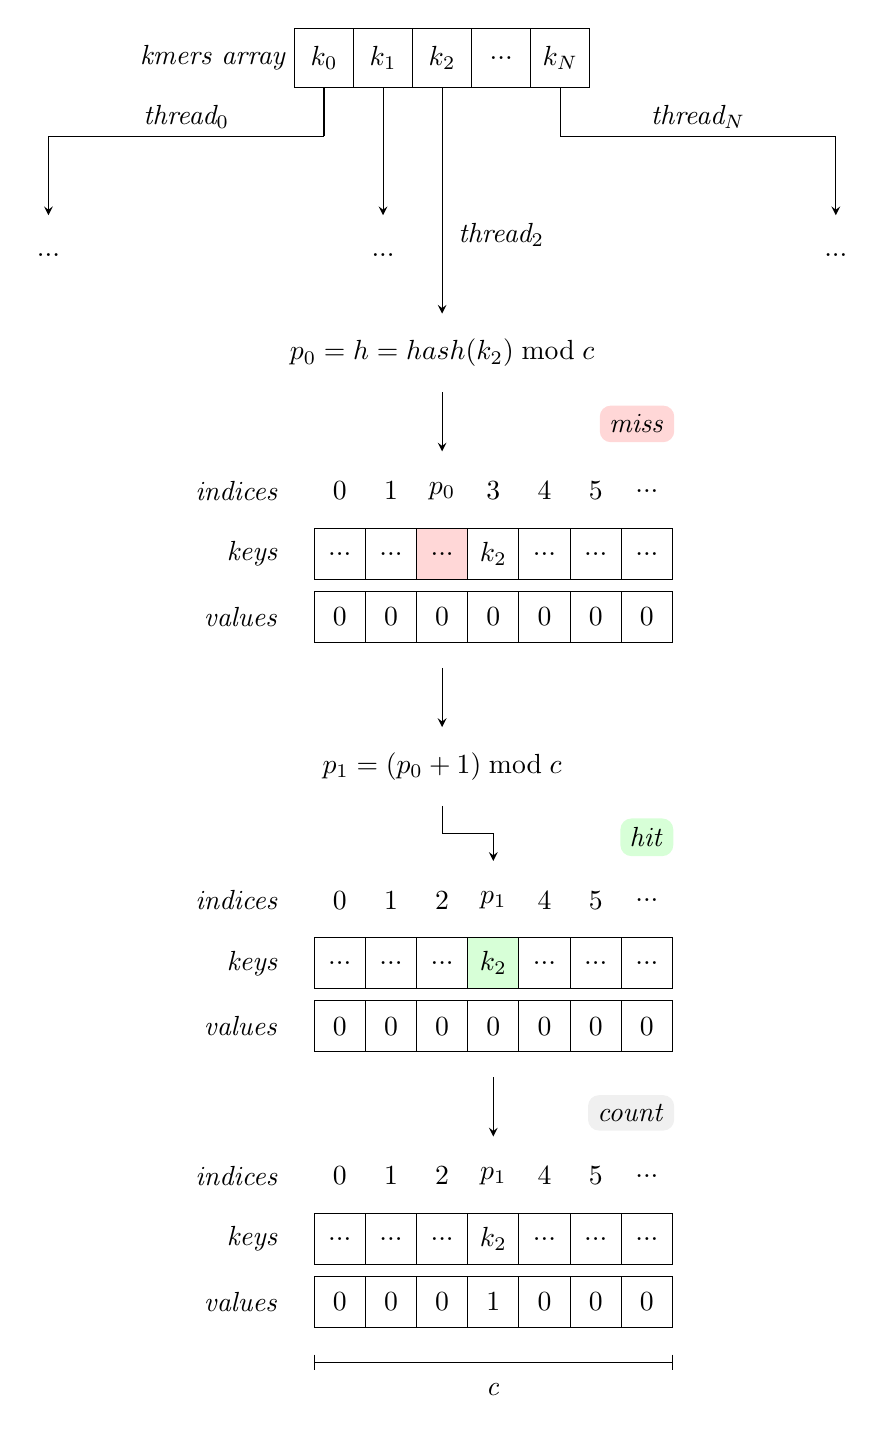
\begin{tikzpicture}
  % in kmers
  \node at(-2.9,0)(){\textit{\smaller{kmers array}}};
  \node at(-1.5,0)[draw,minimum width=0.75cm,minimum height=0.75cm](k0){\smaller{$k_0$}};
  \node at(-.75,0)[draw,minimum width=0.75cm,minimum height=0.75cm](k1){\smaller{$k_1$}};
  \node at(0,0)[draw,minimum width=0.75cm,minimum height=0.75cm](k2){\smaller{$k_2$}};
  \node at(.75,0)[draw,minimum width=0.75cm,minimum height=0.75cm](gap){\smaller{$...$}};
  \node at(1.5,0)[draw,minimum width=0.75cm,minimum height=0.75cm](kn){\smaller{$k_N$}};
  % CUDA threads
  % k0
  \draw [](k0) -- (-1.5,-1);
  \draw [](-1.5,-1) -- (-5,-1);
  \draw [-stealth](-5,-1) -- (-5,-2);
  \node at(-3.25,-.75)(){\textit{\smaller{thread$_0$}}};
  \node at(-5,-2.5)(){...};
  % k1
  \draw [-stealth](k1) -- (-.75,-2);
  \node at(-.75,-2.5)(){...};
  % kn
  \draw [](kn) -- (1.5,-1);
  \draw [](1.5,-1) -- (5,-1);
  \draw [-stealth](5,-1) -- (5,-2);
  \node at(3.25,-.75)(){\textit{\smaller{thread$_N$}}};
  \node at(5,-2.5)(){...};
  % k2
  \draw [-stealth](k2) -- (0,-3.25);
  \node at(.75,-2.25)(){\textit{\smaller{thread$_2$}}};
  % hash
  \node at(0,-3.75)(){\smaller{\textit{$p_0=h=hash(k_2) \bmod c$}}};
  % probe 1
  \draw [-stealth](0,-4.25) -- (0,-5);
  \node at(2.475,-4.65)[fill=misscolor,rounded corners](){\textit{\smaller{miss}}};
  % titles
  \node at(-2.6,-5.5)(){\textit{\smaller{indices}}};
  \node at(-2.4,-6.3)(){\textit{\smaller{keys}}};
  \node at(-2.55,-7.1)(){\textit{\smaller{values}}};
  % indices
  \node at(-1.3,-5.5)[minimum width=0.65cm,minimum height=0.65cm](){\smaller{$0$}};
  \node at(-.65,-5.5)[minimum width=0.65cm,minimum height=0.65cm](){\smaller{$1$}};
  \node at(0,-5.5)[minimum width=0.65cm,minimum height=0.65cm](){\smaller{$p_0$}};
  \node at(.65,-5.5)[minimum width=0.65cm,minimum height=0.65cm](){\smaller{$3$}};
  \node at(1.3,-5.5)[minimum width=0.65cm,minimum height=0.65cm](){\smaller{$4$}};
  \node at(1.95,-5.5)[minimum width=0.65cm,minimum height=0.65cm](){\smaller{$5$}};
  \node at(2.6,-5.5)[minimum width=0.65cm,minimum height=0.65cm](){\smaller{$...$}};
  % keys
  \node at(-1.3,-6.3)[draw,minimum width=0.65cm,minimum height=0.65cm](){\smaller{$...$}};
  \node at(-.65,-6.3)[draw,minimum width=0.65cm,minimum height=0.65cm](){\smaller{$...$}};
  \node at(0,-6.3)[draw,minimum width=0.65cm,minimum height=0.65cm,fill=misscolor](){\smaller{$...$}};
  \node at(.65,-6.3)[draw,minimum width=0.65cm,minimum height=0.65cm](){\smaller{$k_2$}};
  \node at(1.3,-6.3)[draw,minimum width=0.65cm,minimum height=0.65cm](){\smaller{$...$}};
  \node at(1.95,-6.3)[draw,minimum width=0.65cm,minimum height=0.65cm](){\smaller{$...$}};
  \node at(2.6,-6.3)[draw,minimum width=0.65cm,minimum height=0.65cm](){\smaller{$...$}};
  % values
  \node at(-1.3,-7.1)[draw,minimum width=0.65cm,minimum height=0.65cm](){\smaller{$0$}};
  \node at(-.65,-7.1)[draw,minimum width=0.65cm,minimum height=0.65cm](){\smaller{$0$}};
  \node at(0,-7.1)[draw,minimum width=0.65cm,minimum height=0.65cm](){\smaller{$0$}};
  \node at(.65,-7.1)[draw,minimum width=0.65cm,minimum height=0.65cm](){\smaller{$0$}};
  \node at(1.3,-7.1)[draw,minimum width=0.65cm,minimum height=0.65cm](){\smaller{$0$}};
  \node at(1.95,-7.1)[draw,minimum width=0.65cm,minimum height=0.65cm](){\smaller{$0$}};
  \node at(2.6,-7.1)[draw,minimum width=0.65cm,minimum height=0.65cm](){\smaller{$0$}};
  % probe 2
  \draw [-stealth](0,-7.75) -- (0,-8.5);
  \node at(0,-9)(){\smaller{\textit{$p_1=(p_0 + 1) \bmod c$}}};
  \draw [](0,-9.5) -- (0,-9.85);
  \draw [](0,-9.85) -- (.65,-9.85);
  \draw [-stealth](.65,-9.85) -- (.65,-10.2);
  \node at(-2.6,-10.7)(){\textit{\smaller{indices}}};
  \node at(-2.4,-11.5)(){\textit{\smaller{keys}}};
  \node at(-2.55,-12.3)(){\textit{\smaller{values}}};
  \node at(2.6,-9.9)[fill=hitcolor,rounded corners](){\textit{\smaller{hit}}};
  % indices
  \node at(-1.3,-10.7)[minimum width=0.65cm,minimum height=0.65cm](){\smaller{$0$}};
  \node at(-.65,-10.7)[minimum width=0.65cm,minimum height=0.65cm](){\smaller{$1$}};
  \node at(0,-10.7)[minimum width=0.65cm,minimum height=0.65cm](){\smaller{$2$}};
  \node at(.65,-10.7)[minimum width=0.65cm,minimum height=0.65cm](){\smaller{$p_1$}};
  \node at(1.3,-10.7)[minimum width=0.65cm,minimum height=0.65cm](){\smaller{$4$}};
  \node at(1.95,-10.7)[minimum width=0.65cm,minimum height=0.65cm](){\smaller{$5$}};
  \node at(2.6,-10.7)[minimum width=0.65cm,minimum height=0.65cm](){\smaller{$...$}};
  % keys
  \node at(-1.3,-11.5)[draw,minimum width=0.65cm,minimum height=0.65cm](){\smaller{$...$}};
  \node at(-.65,-11.5)[draw,minimum width=0.65cm,minimum height=0.65cm](){\smaller{$...$}};
  \node at(0,-11.5)[draw,minimum width=0.65cm,minimum height=0.65cm](){\smaller{$...$}};
  \node at(.65,-11.5)[draw,minimum width=0.65cm,minimum height=0.65cm,fill=hitcolor](){\smaller{$k_2$}};
  \node at(1.3,-11.5)[draw,minimum width=0.65cm,minimum height=0.65cm](){\smaller{$...$}};
  \node at(1.95,-11.5)[draw,minimum width=0.65cm,minimum height=0.65cm](){\smaller{$...$}};
  \node at(2.6,-11.5)[draw,minimum width=0.65cm,minimum height=0.65cm](){\smaller{$...$}};
  % values
  \node at(-1.3,-12.3)[draw,minimum width=0.65cm,minimum height=0.65cm](){\smaller{$0$}};
  \node at(-.65,-12.3)[draw,minimum width=0.65cm,minimum height=0.65cm](){\smaller{$0$}};
  \node at(0,-12.3)[draw,minimum width=0.65cm,minimum height=0.65cm](){\smaller{$0$}};
  \node at(.65,-12.3)[draw,minimum width=0.65cm,minimum height=0.65cm](){\smaller{$0$}};
  \node at(1.3,-12.3)[draw,minimum width=0.65cm,minimum height=0.65cm](){\smaller{$0$}};
  \node at(1.95,-12.3)[draw,minimum width=0.65cm,minimum height=0.65cm](){\smaller{$0$}};
  \node at(2.6,-12.3)[draw,minimum width=0.65cm,minimum height=0.65cm](){\smaller{$0$}};
  % count
  \draw [-stealth](.65,-12.95) -- (.65,-13.7);
  \node at(-2.6,-14.2)(){\textit{\smaller{indices}}};
  \node at(-2.4,-15)(){\textit{\smaller{keys}}};
  \node at(-2.55,-15.8)(){\textit{\smaller{values}}};
  \node at(2.4,-13.4)[fill=countcolor,rounded corners](){\textit{\smaller{count}}};
  % indices
  \node at(-1.3,-14.2)[minimum width=0.65cm,minimum height=0.65cm](){\smaller{$0$}};
  \node at(-.65,-14.2)[minimum width=0.65cm,minimum height=0.65cm](){\smaller{$1$}};
  \node at(0,-14.2)[minimum width=0.65cm,minimum height=0.65cm](){\smaller{$2$}};
  \node at(.65,-14.2)[minimum width=0.65cm,minimum height=0.65cm](){\smaller{$p_1$}};
  \node at(1.3,-14.2)[minimum width=0.65cm,minimum height=0.65cm](){\smaller{$4$}};
  \node at(1.95,-14.2)[minimum width=0.65cm,minimum height=0.65cm](){\smaller{$5$}};
  \node at(2.6,-14.2)[minimum width=0.65cm,minimum height=0.65cm](){\smaller{$...$}};
  % keys
  \node at(-1.3,-15)[draw,minimum width=0.65cm,minimum height=0.65cm](){\smaller{$...$}};
  \node at(-.65,-15)[draw,minimum width=0.65cm,minimum height=0.65cm](){\smaller{$...$}};
  \node at(0,-15)[draw,minimum width=0.65cm,minimum height=0.65cm](){\smaller{$...$}};
  \node at(.65,-15)[draw,minimum width=0.65cm,minimum height=0.65cm](){\smaller{$k_2$}};
  \node at(1.3,-15)[draw,minimum width=0.65cm,minimum height=0.65cm](){\smaller{$...$}};
  \node at(1.95,-15)[draw,minimum width=0.65cm,minimum height=0.65cm](){\smaller{$...$}};
  \node at(2.6,-15)[draw,minimum width=0.65cm,minimum height=0.65cm](){\smaller{$...$}};
  % values
  \node at(-1.3,-15.8)[draw,minimum width=0.65cm,minimum height=0.65cm](){\smaller{$0$}};
  \node at(-.65,-15.8)[draw,minimum width=0.65cm,minimum height=0.65cm](){\smaller{$0$}};
  \node at(0,-15.8)[draw,minimum width=0.65cm,minimum height=0.65cm](){\smaller{$0$}};
  \node at(.65,-15.8)[draw,minimum width=0.65cm,minimum height=0.65cm](){\smaller{$1$}};
  \node at(1.3,-15.8)[draw,minimum width=0.65cm,minimum height=0.65cm](){\smaller{$0$}};
  \node at(1.95,-15.8)[draw,minimum width=0.65cm,minimum height=0.65cm](){\smaller{$0$}};
  \node at(2.6,-15.8)[draw,minimum width=0.65cm,minimum height=0.65cm](){\smaller{$0$}};
  % capacity
  \draw [](-1.625,-16.57) -- (2.925,-16.57); % -16.57
  \draw [](-1.625,-16.47) -- (-1.625,-16.67); % -16.47, -16.67
  \draw [](2.925,-16.47) -- (2.925,-16.67);
  \node at(.65,-16.92)(c){\smaller{\textit{c}}};
\end{tikzpicture}
}
\caption{
  As an array of \textit{N} 64-bit integer encoded kmers are counted by the hash table, \textit{N} CUDA threads will launch and each will compute the first probe position $p_0$ for its assigned kmer \textit{k}. Then, if the key at slot $p_0$ does not contain \textit{k}, it will continue probing by linearly moving up to the next consecutive slot until either an empty key or \textit{k} observed. If an empty key is observed, the thread terminates without changing any of the hash table's values. If \textit{k} is observed, the current slot's value is incremented.
}
\label{methods:gpu_accelerating_kmer_counting:figures:count_example}
\end{center}
\end{figure}

\paragraph{Integration to Python}
In order to integrate the hash table implemented in C++ using CUDA to Python so that it would be compatible with KAGE, we used pybind11 (introduced in section \ref{background:implementation_tools_and_libraries:pybind11}) to create Python bindings for the C++ class and then wrap the implementation in a Python class.
pybind11 provides easy-to-use macros for this, allowing us to add bindings by simply creating a bindings C++ file and then compiling a module where our C++ functionality is contained.

\begin{figure}[H]
\begin{center}
bindings.cpp
\end{center}
\begin{lstlisting}[language=C++,style=cppcode]
#include <pybind11/pybind11.h>
namespace py = pybind11;

int my_function(int a, int b) {
  return a + b;
}

class MyClass {
public:
  MyClass(int number) : number(number) {}
  int get_number() const { return number; } 
private:
  int number;
};

// Use pybind11's PYBIND11_MODULE macro to create Python bindings for our simple function and class
PYBIND11_MODULE(my_module, m) {
  m.doc() = "Documentation for my module";

  m.def("my_function", &my_function);

  py::class_<MyClass>(m, "MyClass")
    .def(py::init<int>())
    .def("get_number", &MyClass::get_number);
}
\end{lstlisting}
\caption{
  An illustration of how pybind11 can be used to create Python bindings for C++ functions and classes using a simple C++ macro: PYBIND11\_MODULE.
  The C++ project can then be compiled to produce the module that can be imported directly into Python.
  pybind11 takes care of translating common data types automatically, including some data structures such as tuples and lists.
  In addition, pybind11 has specific support for NumPy, making the usage of NumPy arrays seamless.
}
\label{methods:gpu_accelerating_kmer_counting:figures:pybind11_example}
\end{figure}

The produced module is finally wrapped around a Python class that takes care of any transitional details between usage and the C++ interface, such as determining whether to call upon a version of a function that expects NumPy arrays with data allocated in the host's RAM or a CuPy array with data allocated in the GPU's RAM.

The final implementation of this CUDA accelerated hash table can be found and installed at \url{https://github.com/kage-genotyper/cucounter}.

\subsubsection{Assessment}
Include runtime data from the \textit{k}mer counting benchmark test, comparing the CUDA hash table against KAGE's multithreaded CPU version and the GPU hash table from Initial Testing \ref{methods:initial_testing}.
